% !TeX root = main.tex
\lecture{19}{Tue 24 Mar 2026 12:00}{Statistical Physics VI: Energies}

\section{Average Kinetic Energy}
In 3D, we derived last lecture:
\[
    \langle E_k\rangle = \frac{3}{2} k_B T
\]

Each component contributes equally, so:
\[
    E_{kx} = E_{ky} = E_{kz} = \frac{1}{2} k_B T
\]

Remember from the second module of the course we have:
\[
    c = \frac{dQ}{dT}
\]

And the first law of thermodynamics:
\[
    dU = dQ - pdV \implies dQ = dU + pdV
\]

At a constant pressure or volume:
\[
    C_v = \left(\frac{\partial Q}{\partial T}\right)_V = \left(\frac{\partial U}{\partial T}\right)_V
\]

We can define an additional value called Enthalpy (free energy):
\[
    dH = dU + P dV
\]

Hence:
\[
    C_p = \left(\frac{\partial Q}{\partial T}\right)_P = \left(\frac{\partial H}{\partial T}\right)_V
\]

For ideal gases, internal energy comes solely from kinetic energy. As we now have average kinetic energy as a function of $T$, we can now say (for per-atom and per-mole cases respectively):
\[
    C_V = \left(\frac{\partial U}{\partial T}\right)_V = \frac{3}{2} k_B
\]
\[
    C_V = \left(\frac{\partial U}{\partial T}\right)_V = \frac{3}{2} R
\]

This works perfectly for monatomic gases, where Mayer's relation also lets us define $C_P$:
\begin{figure}[H]
    \centering
    
\includegraphics[width=\textwidth]{figures/lec19-01.png}
     \caption{}
\end{figure}
But evidently breaks for diatomic molecules\dots\, They seem to have $C_V = 5R/2$? We'll investigate why later.

\section{Law of Equipartition of Energy}
\begin{tcolorbox}
    The Law of Equipartition says that any substance in equilibrium at temperature $T$ has an average energy of $k_B T / 2$ per \textbf{degree of freedom}.

    \vspace{2mm}

    A \textbf{degree of freedom} is any term in the expression for the energy of the system which has a squared position or squared velocity term.
\end{tcolorbox}

In 1D, our expression for kinetic energy is:
\[
    E_k = \frac{1}{2} mv_x^2 = \frac{1}{2}k_B T \implies C_V = \frac{1}{2}R
\]

And in 3D:
\[
    E_k = \frac{1}{2}mv_x^2 + \frac{1}{2}mv_y^2 + \frac{1}{2}mv_z^2 = \frac{3}{2}k_B T \implies C_V = \frac{3}{2}R
\]

\subsection{Example}

\begin{figure}[H]
    \centering
    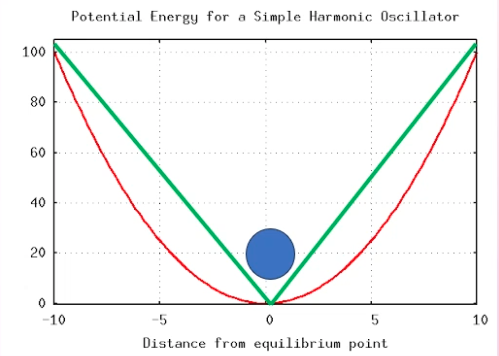
\includegraphics[width=0.75\textwidth]{figures/lec19-02.png}
     \caption{}
\end{figure}

Consider a gas in a harmonic potential, acting as an oscillator in 1D:
\[
    E(V_x, x) = \frac{1}{2}m v_x^2 + \frac{1}{2}kx^2 = k_BT
\]

Or in a linear potential:
\[
    E(v_x, x) = \frac{1}{2}m v_x^2 + Kx = \frac{1}{2}k_B Ts
\]

\subsection{Dulong-Petit Heat Capacity of a Solid}
We model the inter-atomic forces between atoms as springs with spring constant $K$. Each spring has vibrational energy given by:
\[
    E = \frac{1}{2}kx^2 = \frac{1}{2}mv^2 = k_B T
\]

If we assume that the substance forms a perfect cubic lattice where every atom is connected to six other atoms, each spring is shared by two atoms so we say:
\[
    E = 3k_B T \implies c_V = 3R \approx 24.9 \si{mol^{-1} K^{-1}}
\]

This ends up being a surprisingly good fit for pure elements:
\begin{figure}[H]
    \centering
    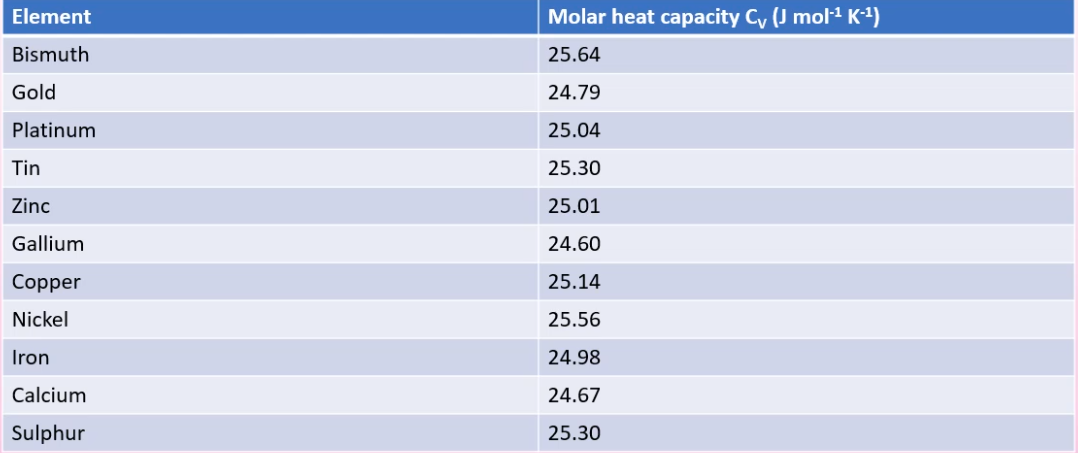
\includegraphics[width=\textwidth]{figures/lec19-03.png}
     \caption{}
\end{figure}

\section{Diatomic Molecules}
Diatomic molecules can be modelled as being connected by a single spring:
\[
    E_\text{vibrational} = \frac{1}{2}kx^2 + \frac{1}{2}m v_x^2 \tag{2 DoF}
\]

However, they are also free to move around the volume in which they occupy, this gives some extra translational energy:
\[
    E_\text{KE} = \frac{1}{2}mv_x^2 + \frac{1}{2}mv_y^2 + \frac{1}{2}mv_z^2 \tag{3 DoF}
\]

Finally, they're also able to rotate around the axis joining them (perpendicularly):
\[
    E_\text{rot} = \frac{1}{2}I \omega^2_y + \frac{1}{2}I \omega^2_z \tag{2 DoF}
\]

In theory this means that a diatomic molecule has 7 degrees of freedom. We saw earlier however that the values for $C_V$ for a diatomic molecule is $C_V = 5R/2$, only implying 5 DoF? Lets look at some actual data:
\begin{figure}[H]
    \centering
    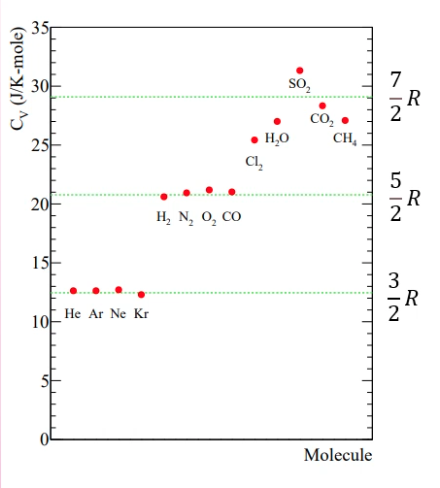
\includegraphics[width=0.75\textwidth]{figures/lec19-04.png}
     \caption{}
\end{figure}

Our monatomic gases behave well, with values close to $3R/2$, but our diatomic gases seem to be more varied, with Chlorine having a much higher value between $5R/2$ and very roughly $7R/2$?

We can't say that our assumption of 7DoF is wrong, because Chlorine sits nicely between them. It means that this cannot, for example, simply lack rotational energy.

The states where a molecule has vibrational energy occurs at larger energies. In order to get a reasonable probability of measuring a state with a certain energy from the Boltzmann factor:

\[
    \Pr(E_i) \propto \exp \left(- \frac{E_i}{k_B T}\right)
\]

We require $k_BT \not\ll E_i$. This gives a transition, where for some temperatures there is some intermediary probability where there's a good chance of measuring particles with and without sufficient energy for the final degrees of freedom. 

This gives a plot like this:
\begin{figure}[H]
    \centering
    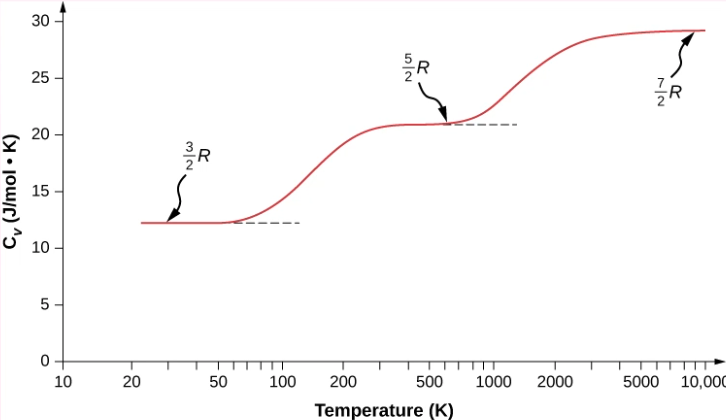
\includegraphics[width=0.75\textwidth]{figures/lec19-05.png}
     \caption{}
\end{figure}

The translational component is always present, as our gas molecules are always present. The vibrational and rotational modes only appear at certain levels where there is sufficient energy to ``unlock'' them.

The degrees of freedom can be considered fully excited if:
\[
    k_BT \gg E_1 - E_0
\]

And if:
\[
    k_BT \ll E_1 - E_0
\]
There is insufficient energy to expect to encounter any molecules with sufficient energy for the motion associated with the degree of freedom, and it is said to be frozen out.